\documentclass[12pt]{article}

\usepackage{fullpage}
\usepackage{multicol,multirow}
\usepackage{tabularx}
\usepackage{ulem}
\usepackage[utf8]{inputenc}
\usepackage[russian]{babel}
\usepackage{amsmath}
\usepackage{amssymb}
\usepackage{graphicx}
\graphicspath{./}
\usepackage{color}
\usepackage{titlesec}

\titleformat{\section}
  {\normalfont\Large\bfseries}{\thesection.}{0.3em}{}

\titleformat{\subsection}
  {\normalfont\large\bfseries}{\thesubsection.}{0.3em}{}

\titlespacing{\section}{0pt}{*2}{*2}
\titlespacing{\subsection}{0pt}{*1}{*1}
\titlespacing{\subsubsection}{0pt}{*0}{*0}
\usepackage{listings}
\lstloadlanguages{Lisp}
\lstset{extendedchars=false,
	breaklines=true,
	breakatwhitespace=true,
	keepspaces = true,
	tabsize=2
}
\begin{document}


\section*{Отчет по лабораторной работе №\,1 
по курсу \guillemotleft  Функциональное программирование\guillemotright}
\begin{flushright}
Студент группы 8О-308 МАИ \textit{Балес Александр}, \textnumero 3 по списку \\
\makebox[7cm]{Контакты: {\tt aleks\_bales@mail.ru} \hfill} \\
\makebox[7cm]{Работа выполнена: 03.03.2016 \hfill} \\
\ \\
Преподаватель: Иванов Дмитрий Анатольевич, доц. каф. 806 \\
\makebox[7cm]{Отчет сдан: \hfill} \\
\makebox[7cm]{Итоговая оценка: \hfill} \\
\makebox[7cm]{Подпись преподавателя: \hfill} \\

\end{flushright}

\section{Тема работы}
Примитивные функции и особые операторы Коммон Лисп.

\section{Цель работы}
Овладеть таким инструментом для решения задач, как примитивные функции и научиться пользоваться особыми операторами.

\section{Задание(вариант 1.41)}
Синус угла (заданного в радианах) можно вычислить следующим образом.
$$sin(x)\approx x$$ приближение при достаточно малых $x$, $$sin(x) = 3sin\dfrac{x}{3} - 4sin^3\dfrac{x}{3}$$ тригонометрическое тождество для уменьшения значения аргумента $sin$.

Будем считать, что угол <<достаточно мал>>, если он не больше $0,1$ радиана.

Запрограммируйте на языке Коммон Лисп функцию, вычисляющую синус по указанной формуле, с использованием рекурсии.
\section{Оборудование студента}
Процессор Intel Core i5-3210 4\,@\,2.5GHz, память: 8192Mb, разрядность системы: 64.

\section{Программное обеспечение}
ОС Ubuntu 14.04, среда GNU Common Lisp 2.6.10

\section{Идея, метод, алгоритм}
Функция {\color{red}\tt{sine}} рекурсивна и работает следующим образом:
\begin{itemize}
\setlength{\itemsep}{-1mm} % уменьшает расстояние между элементами списка
\item если вызвана с аргументом меньшим, чем 0.1 радиан, то вернет аргумент
\item иначе вернет результат $sin(x) = 3sin\dfrac{x}{3} - 4sin^3\dfrac{x}{3}$ с рекурсивным вызовом.
\end{itemize}

\section{Сценарий выполнения работы}
\section{Распечатка программы и её результаты}
\lstinputlisting{./lr1.lsp}
\subsection{Результаты}
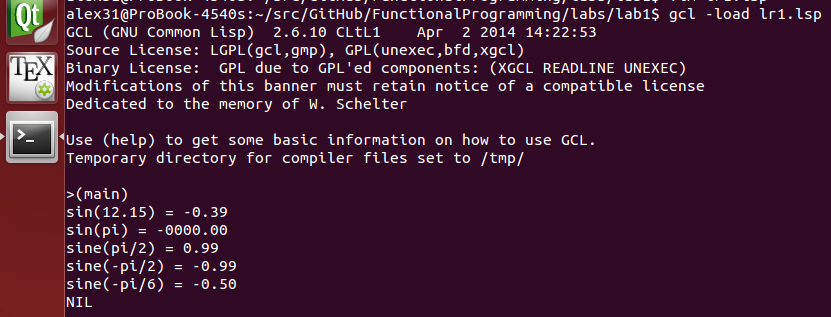
\includegraphics[scale=0.7]{lr1Screen}

%\subsection{Результаты работы}
%\lstinputlisting{./log2.lsp}

\section{Дневник отладки}
\begin{tabular}{|c|p{5cm}|p{5cm}|p{3cm}|}
\hline
Дата & Событие & Действие по исправлению & Примечание \\
\hline
10.03.2016 & 
Некорректная обработка
отрицательного аргумента синуса & 
Проверка на малость значения
аргумента в ф-ии {\color{red}\tt{sine}} заменил 
проверкой модуля аргумента & \\ 
\hline 
10.03.2016 & Оптимизация ф-ии {\color{red}\tt{pow}} & Замена на ф-ию 
{\color{red}\tt{cube}} & Работает за $O(1)$, что быстрее, 
чем $O(lg{N})$ \\ 
\hline
\end{tabular}

\section{Замечания, выводы}
По Мастер Методу следует, что сложность работы данного алгоритма - $O(N\lg{N})$, если же использовать быстрое возведение в степень, то сложность можно понизить до $O(\lg^2N)$. Особым моментом, на мой взгляд, является то, что следует учесть и отрицательные значения аргумента синуса, хотя о них в условии и не упоминалось, этот момент решается благодаря логическому условию {\tt or} в конструкции {\tt if}. Также стоит отметить, что если увеличить точность до $0.001$, то ответ, который выдает программа будет идентичен ответу, который представлен в пример к лабораторной работе. Вид рекурсии - \tt{древовидная}.
\end{document}
